%=====================================================================
%  MMSS Graph Theory : Daily Report + Solutions
%
%  This is the only file you edit day to day.
%  All packages, styles and graph macros live in backend.tex.
%  Cheat sheet for the graph toolkit: top of backend.tex, or readme.txt.
%=====================================================================
\documentclass[11pt]{article}

%settings
\newcommand{\teamname}{[B.A.S.H]}
\newcommand{\reportdate}{\today}
\newcommand{\logopath}{assets/logo.png}  


%=====================================================================
%  backend.tex : MMSS Graph Theory report engine
%
%  DO NOT edit this file for day-to-day reports. Edit main.tex.
%  Touch this file only when you want a NEW macro or a style change.
%  (Makers note : This was really hard to make and I strongly suggest 
%  you dont touch it T-T....)
%  Loaded by main.tex via %=====================================================================
%  backend.tex : MMSS Graph Theory report engine
%
%  DO NOT edit this file for day-to-day reports. Edit main.tex.
%  Touch this file only when you want a NEW macro or a style change.
%  (Makers note : This was really hard to make and I strongly suggest 
%  you dont touch it T-T....)
%  Loaded by main.tex via %=====================================================================
%  backend.tex : MMSS Graph Theory report engine
%
%  DO NOT edit this file for day-to-day reports. Edit main.tex.
%  Touch this file only when you want a NEW macro or a style change.
%  (Makers note : This was really hard to make and I strongly suggest 
%  you dont touch it T-T....)
%  Loaded by main.tex via \input{backend} (after \documentclass).
%
%  Expects (optionally) these to be defined in main.tex BEFORE \input:
%    \teamname    \reportdate    \logopath
%  Fallbacks are provided below, so nothing breaks if you forget.
%
%  ---------------------------------------------------------------
%  GRAPH TOOLKIT CHEAT SHEET  (all calls go INSIDE graphfig/tikzpicture)
%  ---------------------------------------------------------------
%    \gcycle{n}{radius}{prefix}      n vertices on a circle, joined as a cycle
%    \gcyclen{n}{radius}{prefix}     same, vertices labelled 1..n
%    \gcomplete{n}{radius}{prefix}   complete graph K_n on a circle
%    \gbipartite{m}{n}{gap}          complete bipartite K_{m,n}
%                                      handles: left bl1..blm, right br1..brn
%    \gpath{n}{spacing}{prefix}      path on n vertices, left to right
%    \gpetersen                      Petersen graph  (\gpeterson kept as alias)
%                                      handles: outer po0..po4, inner pin0..pin4
%    \gcube{n}                       n x n x n grid cube, oblique 2D projection
%    \gqgon{n}, \gpancake{n}         suprise hidden functions, only use after you 
%                                      learned what it is. 
%
%  Named handles stay live for the rest of the picture, so after a call:
%    \draw[edge,densely dashed] (po0)--(pin2);   or   \node[hv] at (bl1){};
%
%  Vertex styles:  v (filled dot) . ov (open ring) . hv (highlighted hub)
%  Edge style:     edge
%
%  Figure wrapper: \begin{graphfig}[scale]{Label} ... \end{graphfig}
%    {Text} -> centred, titled  [Graph Text]
%    {NUM}  -> centred, auto-numbered  [Graph 1], [Graph 2], ...
%    {}     -> bare, no title, no centring (use to line pictures up side by side)
%=====================================================================

\usepackage[margin=1in,headheight=30pt,headsep=16pt]{geometry}
\usepackage{amsmath,amssymb,amsfonts,amsthm}
\usepackage{enumitem}
\usepackage{fancyhdr}
\usepackage{graphicx}
\usepackage{float}
\usepackage{tikz}
\usepackage{xcolor}
\usetikzlibrary{arrows.meta,calc}


\providecommand{\teamname}{[GROUP NAME]}
\providecommand{\reportdate}{\today}
\providecommand{\logopath}{assets/logo.png}

\pagestyle{fancy}
\fancyhf{}
\renewcommand{\headrulewidth}{0.4pt}
\renewcommand{\footrulewidth}{0pt}
\fancyhead[L]{\raisebox{2pt}{\small\textsc{\teamname}}}
\fancyhead[R]{\expandafter\IfFileExists\expandafter{\logopath}
  {\includegraphics[height=10pt]{\logopath}}{}}
\fancyfoot[C]{\small\thepage}

\fancypagestyle{firstpage}{
  \fancyhf{}
  \renewcommand{\headrulewidth}{0pt}
  \fancyfoot[C]{\small\thepage}
}

\setlength{\parindent}{0pt}
\setlength{\parskip}{6pt}

\newcommand{\divider}{\begin{center}\rule{0.6\textwidth}{0.4pt}\end{center}}

\newtheoremstyle{solstyle}{6pt}{6pt}{}{}{\bfseries}{.}{ }{}
\theoremstyle{solstyle}
\newtheorem*{solution}{Solution}

\newcommand{\WLoG}{WLoG}
\newcommand{\Cn}[1]{C_{#1}}
\newcommand{\Kn}[1]{K_{#1}}
\newcommand{\Kt}[2]{K_{#1,#2}}

\tikzset{
  v/.style ={circle, fill=black, inner sep=1.6pt},
  ov/.style={circle, draw=black, fill=white, line width=0.6pt, inner sep=1.6pt},
  hv/.style={circle, fill=black!55, draw=black, line width=0.6pt, inner sep=2.6pt},
  edge/.style={line width=0.6pt},
}


\newcommand{\gcycle}[3]{
  \foreach \gi in {1,...,#1}{\node[v] (#3\gi) at ({90-(\gi-1)*360/#1}:#2){};}
  \foreach \gi in {1,...,#1}{\pgfmathtruncatemacro{\gj}{mod(\gi,#1)+1}\draw[edge] (#3\gi)--(#3\gj);}
}

\newcommand{\gcyclen}[3]{
  \foreach \gi in {1,...,#1}{
    \pgfmathsetmacro{\gang}{90-(\gi-1)*360/#1}
    \node[v,label={\gang:\gi}] (#3\gi) at (\gang:#2){};}
  \foreach \gi in {1,...,#1}{\pgfmathtruncatemacro{\gj}{mod(\gi,#1)+1}\draw[edge] (#3\gi)--(#3\gj);}
}

\newcommand{\gcomplete}[3]{
  \foreach \gi in {1,...,#1}{\node[v] (#3\gi) at ({90-(\gi-1)*360/#1}:#2){};}
  \foreach \gi in {1,...,#1}{\foreach \gj in {1,...,#1}{\ifnum\gi<\gj\relax\draw[edge] (#3\gi)--(#3\gj);\fi}}
}

\newcommand{\gbipartite}[3]{
  \foreach \gi in {1,...,#1}{\node[v] (bl\gi) at (0,{(#1+1)/2-\gi}){};}
  \foreach \gj in {1,...,#2}{\node[v] (br\gj) at (#3,{(#2+1)/2-\gj}){};}
  \foreach \gi in {1,...,#1}{\foreach \gj in {1,...,#2}{\draw[edge] (bl\gi)--(br\gj);}}
}

\newcommand{\gpath}[3]{
  \foreach \gi in {1,...,#1}{\node[v] (#3\gi) at ({(\gi-1)*#2},0){};}
  \pgfmathtruncatemacro{\gplast}{#1-1}
  \foreach \gi in {1,...,\gplast}{\pgfmathtruncatemacro{\gpk}{\gi+1}\draw[edge] (#3\gi)--(#3\gpk);}
}


\newcommand{\gpetersen}{
  \foreach \gp in {0,...,4}{
    \node[v] (po\gp) at ({90+\gp*72}:2){};
    \node[v] (pin\gp) at ({90+\gp*72}:1){};}
  \foreach \gp in {0,...,4}{
    \pgfmathtruncatemacro{\gpj}{mod(\gp+1,5)}
    \pgfmathtruncatemacro{\gpk}{mod(\gp+2,5)}
    \draw[edge] (po\gp)--(po\gpj);
    \draw[edge] (po\gp)--(pin\gp);
    \draw[edge] (pin\gp)--(pin\gpk);
  }
}
\newcommand{\gpeterson}{\gpetersen}

\newcommand{\gcube}[1]{
  \begin{scope}[x={(1cm,0cm)}, y={(0cm,1cm)}, z={(0.5cm,0.45cm)}]
    \foreach \ci in {0,...,#1}{\draw[edge] (\ci,0,0)--(\ci,#1,0);}
    \foreach \cj in {0,...,#1}{\draw[edge] (0,\cj,0)--(#1,\cj,0);}
    \foreach \ci in {0,...,#1}{\draw[edge] (\ci,#1,0)--(\ci,#1,#1);}
    \foreach \ck in {0,...,#1}{\draw[edge] (0,#1,\ck)--(#1,#1,\ck);}
    \foreach \cj in {0,...,#1}{\draw[edge] (#1,\cj,0)--(#1,\cj,#1);}
    \foreach \ck in {0,...,#1}{\draw[edge] (#1,0,\ck)--(#1,#1,\ck);}
    \foreach \ci in {0,...,#1}{\foreach \cj in {0,...,#1}{\node[v] at (\ci,\cj,0){};}}
    \foreach \ci in {0,...,#1}{\foreach \ck in {0,...,#1}{\node[v] at (\ci,#1,\ck){};}}
    \foreach \cj in {0,...,#1}{\foreach \ck in {0,...,#1}{\node[v] at (#1,\cj,\ck){};}}
  \end{scope}
}

\newcount\pgPlaced
\newcount\pgNf
\newcount\pgTt
\newcommand{\gpancake}[2]{
  \pgNf=1 \pgTt=1
  \loop\ifnum\pgTt<#1 \advance\pgTt by1\relax \multiply\pgNf by\pgTt \repeat
  \edef\pgNfact{\the\pgNf}
  \pgfmathtruncatemacro{\pgTotm}{#1^#1-1}
  \pgPlaced=0
  \foreach \pgI in {0,...,\pgTotm}{
    \gdef\pgPerm{}\xdef\pgUsed{0}\xdef\pgValid{1}
    \foreach \pos in {1,...,#1}{
      \pgfmathtruncatemacro{\pgDig}{Mod(floor(\pgI/(#1^(#1-\pos))),#1)}
      \pgfmathtruncatemacro{\pgBit}{Mod(floor(\pgUsed/(2^\pgDig)),2)}
      \ifnum\pgBit=1 \xdef\pgValid{0}
      \else
        \pgfmathtruncatemacro{\pgNewUsed}{\pgUsed+2^\pgDig}\xdef\pgUsed{\pgNewUsed}
        \pgfmathtruncatemacro{\pgD}{\pgDig+1}\xdef\pgPerm{\pgPerm\pgD}
      \fi}
    \ifnum\pgValid=1
      \pgfmathsetmacro{\pgAng}{90-(\the\pgPlaced)*360/\pgNfact}
      \node[v,label={\pgAng:{\tiny\pgPerm}}] (p\pgPerm) at (\pgAng:#2){};
      \global\advance\pgPlaced by1\relax
    \fi}
  \foreach \pgI in {0,...,\pgTotm}{
    \gdef\pgPerm{}\xdef\pgUsed{0}\xdef\pgValid{1}
    \foreach \pos in {1,...,#1}{
      \pgfmathtruncatemacro{\pgDig}{Mod(floor(\pgI/(#1^(#1-\pos))),#1)}
      \pgfmathtruncatemacro{\pgBit}{Mod(floor(\pgUsed/(2^\pgDig)),2)}
      \ifnum\pgBit=1 \xdef\pgValid{0}
      \else
        \pgfmathtruncatemacro{\pgNewUsed}{\pgUsed+2^\pgDig}\xdef\pgUsed{\pgNewUsed}
        \pgfmathtruncatemacro{\pgD}{\pgDig+1}\xdef\pgPerm{\pgPerm\pgD}
        \expandafter\xdef\csname pgDig\pos\endcsname{\pgD}
      \fi}
    \ifnum\pgValid=1
      \foreach \k in {2,...,#1}{
        \xdef\pgNb{}
        \foreach \j in {1,...,\k}{\xdef\pgNb{\csname pgDig\j\endcsname\pgNb}}
        \ifnum\k<#1
          \foreach \j in {\the\numexpr\k+1\relax,...,#1}{\xdef\pgNb{\pgNb\csname pgDig\j\endcsname}}
        \fi
        \draw[edge] (p\pgPerm)--(p\pgNb);
      }
    \fi}
}




\newcommand{\gqgon}[2]{
  \pgfmathtruncatemacro{\Nm}{2^#1-1}
  \pgfmathtruncatemacro{\nm}{#1-1}
  \foreach \i in {0,...,\Nm}{
    \pgfmathsetmacro{\ang}{90-\i*360/(\Nm+1)}
    \xdef\lbl{}
    \foreach \k in {\nm,...,0}{
      \pgfmathtruncatemacro{\bit}{mod(floor(\i/(2^\k)),2)}
      \xdef\lbl{\lbl\bit}
    }
    \node[v,label={\ang:\scriptsize $\lbl$}] (q\i) at (\ang:#2){};
  }
  \foreach \i in {0,...,\Nm}{
    \foreach \k in {0,...,\nm}{
      \pgfmathtruncatemacro{\bit}{mod(floor(\i/(2^\k)),2)}
      \ifnum\bit=0
        \pgfmathtruncatemacro{\j}{\i+2^\k}
        \draw[edge] (q\i)--(q\j);
      \fi
    }
  }
}


\newcommand{\gclebschedges}{
  \foreach \ci in {0,...,15}{
    \foreach \ck in {0,...,3}{
      \pgfmathtruncatemacro{\cb}{2^\ck}
      \pgfmathtruncatemacro{\cbit}{mod(floor(\ci/\cb),2)}
      \ifnum\cbit=0
        \pgfmathtruncatemacro{\cj}{\ci+\cb}
        \draw[edge] (c\ci)--(c\cj);
      \fi}}
  \foreach \ci in {0,...,7}{
    \pgfmathtruncatemacro{\cj}{15-\ci}
    \draw[edge] (c\ci)--(c\cj);}
}

\newcommand{\gclebsch}[2][0.49]{
  \pgfmathsetmacro{\clbri}{#1*#2}
  \foreach \ci in {0,...,7}{
    \pgfmathtruncatemacro{\cj}{\ci+8}
    \node[v] (c\ci) at ({90-\ci*45}:#2){};
    \node[v] (c\cj) at ({90-\ci*45-22.5}:\clbri){};}
  \gclebschedges
}

\newcommand{\gclebschn}[2][0.49]{
  \pgfmathsetmacro{\clbri}{#1*#2}
  \foreach \ci in {0,...,7}{
    \pgfmathtruncatemacro{\cj}{\ci+8}
    \pgfmathsetmacro{\cao}{90-\ci*45}
    \pgfmathsetmacro{\cai}{90-\ci*45-22.5}
    \xdef\clo{}\xdef\cli{}
    \foreach \ck in {3,2,1,0}{
      \pgfmathtruncatemacro{\cbo}{mod(floor(\ci/(2^\ck)),2)}
      \pgfmathtruncatemacro{\cbi}{mod(floor(\cj/(2^\ck)),2)}
      \xdef\clo{\clo\cbo}\xdef\cli{\cli\cbi}}
    \node[v,label={\cao:{\tiny$\clo$}}] (c\ci) at (\cao:#2){};
    \node[v,label={\cai:{\tiny$\cli$}}] (c\cj) at (\cai:\clbri){};}
  \gclebschedges
}


\newcommand{\newinstructor}[2]{
  \definecolor{#2color}{HTML}{#1}
  \expandafter\newcommand\csname #2\endcsname[1]{
    {\color{#2color}\textbf{#2} : ##1}}}

\newcounter{graphnum}
\newif\ifgfbare
\def\gfEmpty{}
\def\gfNUM{NUM}
\newenvironment{graphfig}[2][1]{
  \def\gftmp{#2}
  \ifx\gftmp\gfEmpty
    \gfbaretrue
  \else
    \gfbarefalse
    \ifx\gftmp\gfNUM
      \stepcounter{graphnum}\edef\gflabel{\arabic{graphnum}}
    \else
      \def\gflabel{#2}
    \fi
  \fi
  \ifgfbare\else\begin{center}\fi
  \begin{tikzpicture}[scale=#1]
}{
  \end{tikzpicture}
  \ifgfbare\else\par\vspace{3pt}\textbf{[Graph \gflabel]}\end{center}\fi
}

\newcommand{\glabel}[1]{\begin{center}\textbf{[Graph #1]}\end{center}} (after \documentclass).
%
%  Expects (optionally) these to be defined in main.tex BEFORE \input:
%    \teamname    \reportdate    \logopath
%  Fallbacks are provided below, so nothing breaks if you forget.
%
%  ---------------------------------------------------------------
%  GRAPH TOOLKIT CHEAT SHEET  (all calls go INSIDE graphfig/tikzpicture)
%  ---------------------------------------------------------------
%    \gcycle{n}{radius}{prefix}      n vertices on a circle, joined as a cycle
%    \gcyclen{n}{radius}{prefix}     same, vertices labelled 1..n
%    \gcomplete{n}{radius}{prefix}   complete graph K_n on a circle
%    \gbipartite{m}{n}{gap}          complete bipartite K_{m,n}
%                                      handles: left bl1..blm, right br1..brn
%    \gpath{n}{spacing}{prefix}      path on n vertices, left to right
%    \gpetersen                      Petersen graph  (\gpeterson kept as alias)
%                                      handles: outer po0..po4, inner pin0..pin4
%    \gcube{n}                       n x n x n grid cube, oblique 2D projection
%    \gqgon{n}, \gpancake{n}         suprise hidden functions, only use after you 
%                                      learned what it is. 
%
%  Named handles stay live for the rest of the picture, so after a call:
%    \draw[edge,densely dashed] (po0)--(pin2);   or   \node[hv] at (bl1){};
%
%  Vertex styles:  v (filled dot) . ov (open ring) . hv (highlighted hub)
%  Edge style:     edge
%
%  Figure wrapper: \begin{graphfig}[scale]{Label} ... \end{graphfig}
%    {Text} -> centred, titled  [Graph Text]
%    {NUM}  -> centred, auto-numbered  [Graph 1], [Graph 2], ...
%    {}     -> bare, no title, no centring (use to line pictures up side by side)
%=====================================================================

\usepackage[margin=1in,headheight=30pt,headsep=16pt]{geometry}
\usepackage{amsmath,amssymb,amsfonts,amsthm}
\usepackage{enumitem}
\usepackage{fancyhdr}
\usepackage{graphicx}
\usepackage{float}
\usepackage{tikz}
\usepackage{xcolor}
\usetikzlibrary{arrows.meta,calc}


\providecommand{\teamname}{[GROUP NAME]}
\providecommand{\reportdate}{\today}
\providecommand{\logopath}{assets/logo.png}

\pagestyle{fancy}
\fancyhf{}
\renewcommand{\headrulewidth}{0.4pt}
\renewcommand{\footrulewidth}{0pt}
\fancyhead[L]{\raisebox{2pt}{\small\textsc{\teamname}}}
\fancyhead[R]{\expandafter\IfFileExists\expandafter{\logopath}
  {\includegraphics[height=10pt]{\logopath}}{}}
\fancyfoot[C]{\small\thepage}

\fancypagestyle{firstpage}{
  \fancyhf{}
  \renewcommand{\headrulewidth}{0pt}
  \fancyfoot[C]{\small\thepage}
}

\setlength{\parindent}{0pt}
\setlength{\parskip}{6pt}

\newcommand{\divider}{\begin{center}\rule{0.6\textwidth}{0.4pt}\end{center}}

\newtheoremstyle{solstyle}{6pt}{6pt}{}{}{\bfseries}{.}{ }{}
\theoremstyle{solstyle}
\newtheorem*{solution}{Solution}

\newcommand{\WLoG}{WLoG}
\newcommand{\Cn}[1]{C_{#1}}
\newcommand{\Kn}[1]{K_{#1}}
\newcommand{\Kt}[2]{K_{#1,#2}}

\tikzset{
  v/.style ={circle, fill=black, inner sep=1.6pt},
  ov/.style={circle, draw=black, fill=white, line width=0.6pt, inner sep=1.6pt},
  hv/.style={circle, fill=black!55, draw=black, line width=0.6pt, inner sep=2.6pt},
  edge/.style={line width=0.6pt},
}


\newcommand{\gcycle}[3]{
  \foreach \gi in {1,...,#1}{\node[v] (#3\gi) at ({90-(\gi-1)*360/#1}:#2){};}
  \foreach \gi in {1,...,#1}{\pgfmathtruncatemacro{\gj}{mod(\gi,#1)+1}\draw[edge] (#3\gi)--(#3\gj);}
}

\newcommand{\gcyclen}[3]{
  \foreach \gi in {1,...,#1}{
    \pgfmathsetmacro{\gang}{90-(\gi-1)*360/#1}
    \node[v,label={\gang:\gi}] (#3\gi) at (\gang:#2){};}
  \foreach \gi in {1,...,#1}{\pgfmathtruncatemacro{\gj}{mod(\gi,#1)+1}\draw[edge] (#3\gi)--(#3\gj);}
}

\newcommand{\gcomplete}[3]{
  \foreach \gi in {1,...,#1}{\node[v] (#3\gi) at ({90-(\gi-1)*360/#1}:#2){};}
  \foreach \gi in {1,...,#1}{\foreach \gj in {1,...,#1}{\ifnum\gi<\gj\relax\draw[edge] (#3\gi)--(#3\gj);\fi}}
}

\newcommand{\gbipartite}[3]{
  \foreach \gi in {1,...,#1}{\node[v] (bl\gi) at (0,{(#1+1)/2-\gi}){};}
  \foreach \gj in {1,...,#2}{\node[v] (br\gj) at (#3,{(#2+1)/2-\gj}){};}
  \foreach \gi in {1,...,#1}{\foreach \gj in {1,...,#2}{\draw[edge] (bl\gi)--(br\gj);}}
}

\newcommand{\gpath}[3]{
  \foreach \gi in {1,...,#1}{\node[v] (#3\gi) at ({(\gi-1)*#2},0){};}
  \pgfmathtruncatemacro{\gplast}{#1-1}
  \foreach \gi in {1,...,\gplast}{\pgfmathtruncatemacro{\gpk}{\gi+1}\draw[edge] (#3\gi)--(#3\gpk);}
}


\newcommand{\gpetersen}{
  \foreach \gp in {0,...,4}{
    \node[v] (po\gp) at ({90+\gp*72}:2){};
    \node[v] (pin\gp) at ({90+\gp*72}:1){};}
  \foreach \gp in {0,...,4}{
    \pgfmathtruncatemacro{\gpj}{mod(\gp+1,5)}
    \pgfmathtruncatemacro{\gpk}{mod(\gp+2,5)}
    \draw[edge] (po\gp)--(po\gpj);
    \draw[edge] (po\gp)--(pin\gp);
    \draw[edge] (pin\gp)--(pin\gpk);
  }
}
\newcommand{\gpeterson}{\gpetersen}

\newcommand{\gcube}[1]{
  \begin{scope}[x={(1cm,0cm)}, y={(0cm,1cm)}, z={(0.5cm,0.45cm)}]
    \foreach \ci in {0,...,#1}{\draw[edge] (\ci,0,0)--(\ci,#1,0);}
    \foreach \cj in {0,...,#1}{\draw[edge] (0,\cj,0)--(#1,\cj,0);}
    \foreach \ci in {0,...,#1}{\draw[edge] (\ci,#1,0)--(\ci,#1,#1);}
    \foreach \ck in {0,...,#1}{\draw[edge] (0,#1,\ck)--(#1,#1,\ck);}
    \foreach \cj in {0,...,#1}{\draw[edge] (#1,\cj,0)--(#1,\cj,#1);}
    \foreach \ck in {0,...,#1}{\draw[edge] (#1,0,\ck)--(#1,#1,\ck);}
    \foreach \ci in {0,...,#1}{\foreach \cj in {0,...,#1}{\node[v] at (\ci,\cj,0){};}}
    \foreach \ci in {0,...,#1}{\foreach \ck in {0,...,#1}{\node[v] at (\ci,#1,\ck){};}}
    \foreach \cj in {0,...,#1}{\foreach \ck in {0,...,#1}{\node[v] at (#1,\cj,\ck){};}}
  \end{scope}
}

\newcount\pgPlaced
\newcount\pgNf
\newcount\pgTt
\newcommand{\gpancake}[2]{
  \pgNf=1 \pgTt=1
  \loop\ifnum\pgTt<#1 \advance\pgTt by1\relax \multiply\pgNf by\pgTt \repeat
  \edef\pgNfact{\the\pgNf}
  \pgfmathtruncatemacro{\pgTotm}{#1^#1-1}
  \pgPlaced=0
  \foreach \pgI in {0,...,\pgTotm}{
    \gdef\pgPerm{}\xdef\pgUsed{0}\xdef\pgValid{1}
    \foreach \pos in {1,...,#1}{
      \pgfmathtruncatemacro{\pgDig}{Mod(floor(\pgI/(#1^(#1-\pos))),#1)}
      \pgfmathtruncatemacro{\pgBit}{Mod(floor(\pgUsed/(2^\pgDig)),2)}
      \ifnum\pgBit=1 \xdef\pgValid{0}
      \else
        \pgfmathtruncatemacro{\pgNewUsed}{\pgUsed+2^\pgDig}\xdef\pgUsed{\pgNewUsed}
        \pgfmathtruncatemacro{\pgD}{\pgDig+1}\xdef\pgPerm{\pgPerm\pgD}
      \fi}
    \ifnum\pgValid=1
      \pgfmathsetmacro{\pgAng}{90-(\the\pgPlaced)*360/\pgNfact}
      \node[v,label={\pgAng:{\tiny\pgPerm}}] (p\pgPerm) at (\pgAng:#2){};
      \global\advance\pgPlaced by1\relax
    \fi}
  \foreach \pgI in {0,...,\pgTotm}{
    \gdef\pgPerm{}\xdef\pgUsed{0}\xdef\pgValid{1}
    \foreach \pos in {1,...,#1}{
      \pgfmathtruncatemacro{\pgDig}{Mod(floor(\pgI/(#1^(#1-\pos))),#1)}
      \pgfmathtruncatemacro{\pgBit}{Mod(floor(\pgUsed/(2^\pgDig)),2)}
      \ifnum\pgBit=1 \xdef\pgValid{0}
      \else
        \pgfmathtruncatemacro{\pgNewUsed}{\pgUsed+2^\pgDig}\xdef\pgUsed{\pgNewUsed}
        \pgfmathtruncatemacro{\pgD}{\pgDig+1}\xdef\pgPerm{\pgPerm\pgD}
        \expandafter\xdef\csname pgDig\pos\endcsname{\pgD}
      \fi}
    \ifnum\pgValid=1
      \foreach \k in {2,...,#1}{
        \xdef\pgNb{}
        \foreach \j in {1,...,\k}{\xdef\pgNb{\csname pgDig\j\endcsname\pgNb}}
        \ifnum\k<#1
          \foreach \j in {\the\numexpr\k+1\relax,...,#1}{\xdef\pgNb{\pgNb\csname pgDig\j\endcsname}}
        \fi
        \draw[edge] (p\pgPerm)--(p\pgNb);
      }
    \fi}
}




\newcommand{\gqgon}[2]{
  \pgfmathtruncatemacro{\Nm}{2^#1-1}
  \pgfmathtruncatemacro{\nm}{#1-1}
  \foreach \i in {0,...,\Nm}{
    \pgfmathsetmacro{\ang}{90-\i*360/(\Nm+1)}
    \xdef\lbl{}
    \foreach \k in {\nm,...,0}{
      \pgfmathtruncatemacro{\bit}{mod(floor(\i/(2^\k)),2)}
      \xdef\lbl{\lbl\bit}
    }
    \node[v,label={\ang:\scriptsize $\lbl$}] (q\i) at (\ang:#2){};
  }
  \foreach \i in {0,...,\Nm}{
    \foreach \k in {0,...,\nm}{
      \pgfmathtruncatemacro{\bit}{mod(floor(\i/(2^\k)),2)}
      \ifnum\bit=0
        \pgfmathtruncatemacro{\j}{\i+2^\k}
        \draw[edge] (q\i)--(q\j);
      \fi
    }
  }
}


\newcommand{\gclebschedges}{
  \foreach \ci in {0,...,15}{
    \foreach \ck in {0,...,3}{
      \pgfmathtruncatemacro{\cb}{2^\ck}
      \pgfmathtruncatemacro{\cbit}{mod(floor(\ci/\cb),2)}
      \ifnum\cbit=0
        \pgfmathtruncatemacro{\cj}{\ci+\cb}
        \draw[edge] (c\ci)--(c\cj);
      \fi}}
  \foreach \ci in {0,...,7}{
    \pgfmathtruncatemacro{\cj}{15-\ci}
    \draw[edge] (c\ci)--(c\cj);}
}

\newcommand{\gclebsch}[2][0.49]{
  \pgfmathsetmacro{\clbri}{#1*#2}
  \foreach \ci in {0,...,7}{
    \pgfmathtruncatemacro{\cj}{\ci+8}
    \node[v] (c\ci) at ({90-\ci*45}:#2){};
    \node[v] (c\cj) at ({90-\ci*45-22.5}:\clbri){};}
  \gclebschedges
}

\newcommand{\gclebschn}[2][0.49]{
  \pgfmathsetmacro{\clbri}{#1*#2}
  \foreach \ci in {0,...,7}{
    \pgfmathtruncatemacro{\cj}{\ci+8}
    \pgfmathsetmacro{\cao}{90-\ci*45}
    \pgfmathsetmacro{\cai}{90-\ci*45-22.5}
    \xdef\clo{}\xdef\cli{}
    \foreach \ck in {3,2,1,0}{
      \pgfmathtruncatemacro{\cbo}{mod(floor(\ci/(2^\ck)),2)}
      \pgfmathtruncatemacro{\cbi}{mod(floor(\cj/(2^\ck)),2)}
      \xdef\clo{\clo\cbo}\xdef\cli{\cli\cbi}}
    \node[v,label={\cao:{\tiny$\clo$}}] (c\ci) at (\cao:#2){};
    \node[v,label={\cai:{\tiny$\cli$}}] (c\cj) at (\cai:\clbri){};}
  \gclebschedges
}


\newcommand{\newinstructor}[2]{
  \definecolor{#2color}{HTML}{#1}
  \expandafter\newcommand\csname #2\endcsname[1]{
    {\color{#2color}\textbf{#2} : ##1}}}

\newcounter{graphnum}
\newif\ifgfbare
\def\gfEmpty{}
\def\gfNUM{NUM}
\newenvironment{graphfig}[2][1]{
  \def\gftmp{#2}
  \ifx\gftmp\gfEmpty
    \gfbaretrue
  \else
    \gfbarefalse
    \ifx\gftmp\gfNUM
      \stepcounter{graphnum}\edef\gflabel{\arabic{graphnum}}
    \else
      \def\gflabel{#2}
    \fi
  \fi
  \ifgfbare\else\begin{center}\fi
  \begin{tikzpicture}[scale=#1]
}{
  \end{tikzpicture}
  \ifgfbare\else\par\vspace{3pt}\textbf{[Graph \gflabel]}\end{center}\fi
}

\newcommand{\glabel}[1]{\begin{center}\textbf{[Graph #1]}\end{center}} (after \documentclass).
%
%  Expects (optionally) these to be defined in main.tex BEFORE \input:
%    \teamname    \reportdate    \logopath
%  Fallbacks are provided below, so nothing breaks if you forget.
%
%  ---------------------------------------------------------------
%  GRAPH TOOLKIT CHEAT SHEET  (all calls go INSIDE graphfig/tikzpicture)
%  ---------------------------------------------------------------
%    \gcycle{n}{radius}{prefix}      n vertices on a circle, joined as a cycle
%    \gcyclen{n}{radius}{prefix}     same, vertices labelled 1..n
%    \gcomplete{n}{radius}{prefix}   complete graph K_n on a circle
%    \gbipartite{m}{n}{gap}          complete bipartite K_{m,n}
%                                      handles: left bl1..blm, right br1..brn
%    \gpath{n}{spacing}{prefix}      path on n vertices, left to right
%    \gpetersen                      Petersen graph  (\gpeterson kept as alias)
%                                      handles: outer po0..po4, inner pin0..pin4
%    \gcube{n}                       n x n x n grid cube, oblique 2D projection
%    \gqgon{n}, \gpancake{n}         suprise hidden functions, only use after you 
%                                      learned what it is. 
%
%  Named handles stay live for the rest of the picture, so after a call:
%    \draw[edge,densely dashed] (po0)--(pin2);   or   \node[hv] at (bl1){};
%
%  Vertex styles:  v (filled dot) . ov (open ring) . hv (highlighted hub)
%  Edge style:     edge
%
%  Figure wrapper: \begin{graphfig}[scale]{Label} ... \end{graphfig}
%    {Text} -> centred, titled  [Graph Text]
%    {NUM}  -> centred, auto-numbered  [Graph 1], [Graph 2], ...
%    {}     -> bare, no title, no centring (use to line pictures up side by side)
%=====================================================================

\usepackage[margin=1in,headheight=30pt,headsep=16pt]{geometry}
\usepackage{amsmath,amssymb,amsfonts,amsthm}
\usepackage{enumitem}
\usepackage{fancyhdr}
\usepackage{graphicx}
\usepackage{float}
\usepackage{tikz}
\usepackage{xcolor}
\usetikzlibrary{arrows.meta,calc}


\providecommand{\teamname}{[GROUP NAME]}
\providecommand{\reportdate}{\today}
\providecommand{\logopath}{assets/logo.png}

\pagestyle{fancy}
\fancyhf{}
\renewcommand{\headrulewidth}{0.4pt}
\renewcommand{\footrulewidth}{0pt}
\fancyhead[L]{\raisebox{2pt}{\small\textsc{\teamname}}}
\fancyhead[R]{\expandafter\IfFileExists\expandafter{\logopath}
  {\includegraphics[height=10pt]{\logopath}}{}}
\fancyfoot[C]{\small\thepage}

\fancypagestyle{firstpage}{
  \fancyhf{}
  \renewcommand{\headrulewidth}{0pt}
  \fancyfoot[C]{\small\thepage}
}

\setlength{\parindent}{0pt}
\setlength{\parskip}{6pt}

\newcommand{\divider}{\begin{center}\rule{0.6\textwidth}{0.4pt}\end{center}}

\newtheoremstyle{solstyle}{6pt}{6pt}{}{}{\bfseries}{.}{ }{}
\theoremstyle{solstyle}
\newtheorem*{solution}{Solution}

\newcommand{\WLoG}{WLoG}
\newcommand{\Cn}[1]{C_{#1}}
\newcommand{\Kn}[1]{K_{#1}}
\newcommand{\Kt}[2]{K_{#1,#2}}

\tikzset{
  v/.style ={circle, fill=black, inner sep=1.6pt},
  ov/.style={circle, draw=black, fill=white, line width=0.6pt, inner sep=1.6pt},
  hv/.style={circle, fill=black!55, draw=black, line width=0.6pt, inner sep=2.6pt},
  edge/.style={line width=0.6pt},
}


\newcommand{\gcycle}[3]{
  \foreach \gi in {1,...,#1}{\node[v] (#3\gi) at ({90-(\gi-1)*360/#1}:#2){};}
  \foreach \gi in {1,...,#1}{\pgfmathtruncatemacro{\gj}{mod(\gi,#1)+1}\draw[edge] (#3\gi)--(#3\gj);}
}

\newcommand{\gcyclen}[3]{
  \foreach \gi in {1,...,#1}{
    \pgfmathsetmacro{\gang}{90-(\gi-1)*360/#1}
    \node[v,label={\gang:\gi}] (#3\gi) at (\gang:#2){};}
  \foreach \gi in {1,...,#1}{\pgfmathtruncatemacro{\gj}{mod(\gi,#1)+1}\draw[edge] (#3\gi)--(#3\gj);}
}

\newcommand{\gcomplete}[3]{
  \foreach \gi in {1,...,#1}{\node[v] (#3\gi) at ({90-(\gi-1)*360/#1}:#2){};}
  \foreach \gi in {1,...,#1}{\foreach \gj in {1,...,#1}{\ifnum\gi<\gj\relax\draw[edge] (#3\gi)--(#3\gj);\fi}}
}

\newcommand{\gbipartite}[3]{
  \foreach \gi in {1,...,#1}{\node[v] (bl\gi) at (0,{(#1+1)/2-\gi}){};}
  \foreach \gj in {1,...,#2}{\node[v] (br\gj) at (#3,{(#2+1)/2-\gj}){};}
  \foreach \gi in {1,...,#1}{\foreach \gj in {1,...,#2}{\draw[edge] (bl\gi)--(br\gj);}}
}

\newcommand{\gpath}[3]{
  \foreach \gi in {1,...,#1}{\node[v] (#3\gi) at ({(\gi-1)*#2},0){};}
  \pgfmathtruncatemacro{\gplast}{#1-1}
  \foreach \gi in {1,...,\gplast}{\pgfmathtruncatemacro{\gpk}{\gi+1}\draw[edge] (#3\gi)--(#3\gpk);}
}


\newcommand{\gpetersen}{
  \foreach \gp in {0,...,4}{
    \node[v] (po\gp) at ({90+\gp*72}:2){};
    \node[v] (pin\gp) at ({90+\gp*72}:1){};}
  \foreach \gp in {0,...,4}{
    \pgfmathtruncatemacro{\gpj}{mod(\gp+1,5)}
    \pgfmathtruncatemacro{\gpk}{mod(\gp+2,5)}
    \draw[edge] (po\gp)--(po\gpj);
    \draw[edge] (po\gp)--(pin\gp);
    \draw[edge] (pin\gp)--(pin\gpk);
  }
}
\newcommand{\gpeterson}{\gpetersen}

\newcommand{\gcube}[1]{
  \begin{scope}[x={(1cm,0cm)}, y={(0cm,1cm)}, z={(0.5cm,0.45cm)}]
    \foreach \ci in {0,...,#1}{\draw[edge] (\ci,0,0)--(\ci,#1,0);}
    \foreach \cj in {0,...,#1}{\draw[edge] (0,\cj,0)--(#1,\cj,0);}
    \foreach \ci in {0,...,#1}{\draw[edge] (\ci,#1,0)--(\ci,#1,#1);}
    \foreach \ck in {0,...,#1}{\draw[edge] (0,#1,\ck)--(#1,#1,\ck);}
    \foreach \cj in {0,...,#1}{\draw[edge] (#1,\cj,0)--(#1,\cj,#1);}
    \foreach \ck in {0,...,#1}{\draw[edge] (#1,0,\ck)--(#1,#1,\ck);}
    \foreach \ci in {0,...,#1}{\foreach \cj in {0,...,#1}{\node[v] at (\ci,\cj,0){};}}
    \foreach \ci in {0,...,#1}{\foreach \ck in {0,...,#1}{\node[v] at (\ci,#1,\ck){};}}
    \foreach \cj in {0,...,#1}{\foreach \ck in {0,...,#1}{\node[v] at (#1,\cj,\ck){};}}
  \end{scope}
}

\newcount\pgPlaced
\newcount\pgNf
\newcount\pgTt
\newcommand{\gpancake}[2]{
  \pgNf=1 \pgTt=1
  \loop\ifnum\pgTt<#1 \advance\pgTt by1\relax \multiply\pgNf by\pgTt \repeat
  \edef\pgNfact{\the\pgNf}
  \pgfmathtruncatemacro{\pgTotm}{#1^#1-1}
  \pgPlaced=0
  \foreach \pgI in {0,...,\pgTotm}{
    \gdef\pgPerm{}\xdef\pgUsed{0}\xdef\pgValid{1}
    \foreach \pos in {1,...,#1}{
      \pgfmathtruncatemacro{\pgDig}{Mod(floor(\pgI/(#1^(#1-\pos))),#1)}
      \pgfmathtruncatemacro{\pgBit}{Mod(floor(\pgUsed/(2^\pgDig)),2)}
      \ifnum\pgBit=1 \xdef\pgValid{0}
      \else
        \pgfmathtruncatemacro{\pgNewUsed}{\pgUsed+2^\pgDig}\xdef\pgUsed{\pgNewUsed}
        \pgfmathtruncatemacro{\pgD}{\pgDig+1}\xdef\pgPerm{\pgPerm\pgD}
      \fi}
    \ifnum\pgValid=1
      \pgfmathsetmacro{\pgAng}{90-(\the\pgPlaced)*360/\pgNfact}
      \node[v,label={\pgAng:{\tiny\pgPerm}}] (p\pgPerm) at (\pgAng:#2){};
      \global\advance\pgPlaced by1\relax
    \fi}
  \foreach \pgI in {0,...,\pgTotm}{
    \gdef\pgPerm{}\xdef\pgUsed{0}\xdef\pgValid{1}
    \foreach \pos in {1,...,#1}{
      \pgfmathtruncatemacro{\pgDig}{Mod(floor(\pgI/(#1^(#1-\pos))),#1)}
      \pgfmathtruncatemacro{\pgBit}{Mod(floor(\pgUsed/(2^\pgDig)),2)}
      \ifnum\pgBit=1 \xdef\pgValid{0}
      \else
        \pgfmathtruncatemacro{\pgNewUsed}{\pgUsed+2^\pgDig}\xdef\pgUsed{\pgNewUsed}
        \pgfmathtruncatemacro{\pgD}{\pgDig+1}\xdef\pgPerm{\pgPerm\pgD}
        \expandafter\xdef\csname pgDig\pos\endcsname{\pgD}
      \fi}
    \ifnum\pgValid=1
      \foreach \k in {2,...,#1}{
        \xdef\pgNb{}
        \foreach \j in {1,...,\k}{\xdef\pgNb{\csname pgDig\j\endcsname\pgNb}}
        \ifnum\k<#1
          \foreach \j in {\the\numexpr\k+1\relax,...,#1}{\xdef\pgNb{\pgNb\csname pgDig\j\endcsname}}
        \fi
        \draw[edge] (p\pgPerm)--(p\pgNb);
      }
    \fi}
}




\newcommand{\gqgon}[2]{
  \pgfmathtruncatemacro{\Nm}{2^#1-1}
  \pgfmathtruncatemacro{\nm}{#1-1}
  \foreach \i in {0,...,\Nm}{
    \pgfmathsetmacro{\ang}{90-\i*360/(\Nm+1)}
    \xdef\lbl{}
    \foreach \k in {\nm,...,0}{
      \pgfmathtruncatemacro{\bit}{mod(floor(\i/(2^\k)),2)}
      \xdef\lbl{\lbl\bit}
    }
    \node[v,label={\ang:\scriptsize $\lbl$}] (q\i) at (\ang:#2){};
  }
  \foreach \i in {0,...,\Nm}{
    \foreach \k in {0,...,\nm}{
      \pgfmathtruncatemacro{\bit}{mod(floor(\i/(2^\k)),2)}
      \ifnum\bit=0
        \pgfmathtruncatemacro{\j}{\i+2^\k}
        \draw[edge] (q\i)--(q\j);
      \fi
    }
  }
}


\newcommand{\gclebschedges}{
  \foreach \ci in {0,...,15}{
    \foreach \ck in {0,...,3}{
      \pgfmathtruncatemacro{\cb}{2^\ck}
      \pgfmathtruncatemacro{\cbit}{mod(floor(\ci/\cb),2)}
      \ifnum\cbit=0
        \pgfmathtruncatemacro{\cj}{\ci+\cb}
        \draw[edge] (c\ci)--(c\cj);
      \fi}}
  \foreach \ci in {0,...,7}{
    \pgfmathtruncatemacro{\cj}{15-\ci}
    \draw[edge] (c\ci)--(c\cj);}
}

\newcommand{\gclebsch}[2][0.49]{
  \pgfmathsetmacro{\clbri}{#1*#2}
  \foreach \ci in {0,...,7}{
    \pgfmathtruncatemacro{\cj}{\ci+8}
    \node[v] (c\ci) at ({90-\ci*45}:#2){};
    \node[v] (c\cj) at ({90-\ci*45-22.5}:\clbri){};}
  \gclebschedges
}

\newcommand{\gclebschn}[2][0.49]{
  \pgfmathsetmacro{\clbri}{#1*#2}
  \foreach \ci in {0,...,7}{
    \pgfmathtruncatemacro{\cj}{\ci+8}
    \pgfmathsetmacro{\cao}{90-\ci*45}
    \pgfmathsetmacro{\cai}{90-\ci*45-22.5}
    \xdef\clo{}\xdef\cli{}
    \foreach \ck in {3,2,1,0}{
      \pgfmathtruncatemacro{\cbo}{mod(floor(\ci/(2^\ck)),2)}
      \pgfmathtruncatemacro{\cbi}{mod(floor(\cj/(2^\ck)),2)}
      \xdef\clo{\clo\cbo}\xdef\cli{\cli\cbi}}
    \node[v,label={\cao:{\tiny$\clo$}}] (c\ci) at (\cao:#2){};
    \node[v,label={\cai:{\tiny$\cli$}}] (c\cj) at (\cai:\clbri){};}
  \gclebschedges
}


\newcommand{\newinstructor}[2]{
  \definecolor{#2color}{HTML}{#1}
  \expandafter\newcommand\csname #2\endcsname[1]{
    {\color{#2color}\textbf{#2} : ##1}}}

\newcounter{graphnum}
\newif\ifgfbare
\def\gfEmpty{}
\def\gfNUM{NUM}
\newenvironment{graphfig}[2][1]{
  \def\gftmp{#2}
  \ifx\gftmp\gfEmpty
    \gfbaretrue
  \else
    \gfbarefalse
    \ifx\gftmp\gfNUM
      \stepcounter{graphnum}\edef\gflabel{\arabic{graphnum}}
    \else
      \def\gflabel{#2}
    \fi
  \fi
  \ifgfbare\else\begin{center}\fi
  \begin{tikzpicture}[scale=#1]
}{
  \end{tikzpicture}
  \ifgfbare\else\par\vspace{3pt}\textbf{[Graph \gflabel]}\end{center}\fi
}

\newcommand{\glabel}[1]{\begin{center}\textbf{[Graph #1]}\end{center}}

\begin{document}
\thispagestyle{firstpage}

%frontmatter
\noindent\textbf{\teamname}\hfill\textbf{\reportdate}
\definecolor{djs}{rgb}{0.6, 0.4, 0.8}
\noindent\textbf{Clarifier:} Henry\\
\textbf{Manager:} Seungwon\\
\textbf{Reporter:} Rachel \& Aadya\\
\textbf{Skeptic:} Benjamin

\textbf{Report:} Today, felt pretty relaxed as we got many problems done and worked together. Number 1 and 2 were quick, in general, though they required some discussion/time to make the graphs. 3 and 4 were also done fast since many of the ideas were similar to 1/2 and to examples in-class. For number 5, we were able to illustrate our example from in-class, but we did not have enough time to prove each of the conditions. 6 was also easier, so we finished that alongside 7 \color{blue} hehehehehe \color{black} and part of question 8 (still have to prove the necessary condition). Number 9 was also simple to write-up, so we had time to create a graph for 10. Finally, we completed 12 and 15c. Thank you to everyone who made this program possible!  
\newline NOW ONTO THE MORE IMPORTANT RACHEL ADDITION: 
\newline So like someone in this group (I am not a snitch) gave me some chewing gum so that I may be able to write their report for them. The person in the group was busy hanging out with their friend Parabola who they met at a function once. Anyways, our group worked with some other people from another group (Spies I fear) to solve our problems and then we went back to our respective groups for the write up process. It was a pretty chill day. I mean we got side tracked a little with doing the dotted line thingy-thing on the chalkboards but who wouldn't when we got like 10 new sticks of chalk! Anyways, we all really loved the course (hance why I am here four years later still being a reporter) and thank you all for being here for us these past two weeks!!
\color{djs} I never thought that this part of the homework would get all meta. (Original meaning of the word, not the company).  But there we are. I paid the money, I take the ride. \color{black}


% Instructor comments, if any:
%   \newinstructor{FF6600}{john}   in the settings area or right here
%   then use   \john{lorem ipsum}
%=====================================================================

\divider

\textbf{SOLUTIONS \& PROOFS:}\\
% Any extra notes to the reader go here.
Without Loss of Generality is abbreviated as \WLoG{} within this document.

%problems
\begin{enumerate}[leftmargin=*]
    \item $n=20$, Brualdi graphs where ${a,b}$ is an edge IFF $a+b$ is odd. \color{red}Great work!\color{black}
    \begin{graphfig}{NUM}
        \node [ov] (a1) at (0:5){$1$};
        \node [ov] (a2) at (18:5){$2$};
        \node [ov] (a3) at (36:5){$3$};
        \node [ov] (a4) at (54:5){$4$};
        \node [ov] (a5) at (72:5){$5$};
        \node [ov] (a6) at (90:5){$6$};
        \node [ov] (a7) at (108:5){$7$};
        \node [ov] (a8) at (126:5){$8$};
        \node [ov] (a9) at (144:5){$9$};
        \node [ov] (a10) at (162:5){$10$};
        \node [ov] (a11) at (180:5){$11$};
        \node [ov] (a12) at (198:5){$12$};
        \node [ov] (a13) at (216:5){$13$};
        \node [ov] (a14) at (234:5){$14$};
        \node [ov] (a15) at (252:5){$15$};
        \node [ov] (a16) at (270:5){$16$};
        \node [ov] (a17) at (288:5){$17$};
        \node [ov] (a18) at (306:5){$18$};
        \node [ov] (a19) at (324:5){$19$};
        \node [ov] (a20) at (342:5){$20$};
        \draw (a1)--(a2)--(a3)--(a4)--(a5)--(a6)--(a7)--(a8)--(a9)--(a10)--(a11)--(a12)--(a13)--(a14)--(a15)--(a16)--(a17)--(a18)--(a19)--(a20)--(a1) (a1)--(a4) (a1)--(a6) (a1)--(a8) (a1)--(a10) (a1)--(a12) (a1)--(a14) (a1)--(a16) (a1)--(a18) (a3)--(a4) (a3)--(a6) (a3)--(a8) (a3)--(a10) (a3)--(a12) (a3)--(a14) (a3)--(a16) (a3)--(a18) (a3)--(a20) (a5)--(a2) (a5)--(a4) (a5)--(a6) (a5)--(a8) (a5)--(a10) (a5)--(a12) (a5)--(a14) (a5)--(a16) (a5)--(a18) (a5)--(a20) (a7)--(a2) (a7)--(a4) (a7)--(a6) (a7)--(a8) (a7)--(a10) (a7)--(a12) (a7)--(a14) (a7)--(a16) (a7)--(a18) (a7)--(a20) (a9)--(a2) (a9)--(a4) (a9)--(a6) (a9)--(a8) (a9)--(a10) (a9)--(a12) (a9)--(a14) (a9)--(a16) (a9)--(a18) (a9)--(a20) (a11)--(a2) (a11)--(a4) (a11)--(a6) (a11)--(a8) (a11)--(a10) (a11)--(a12) (a11)--(a14) (a11)--(a16) (a11)--(a18) (a11)--(a20) (a13)--(a2) (a13)--(a4) (a13)--(a6) (a13)--(a8) (a13)--(a10) (a13)--(a12) (a13)--(a14) (a13)--(a16) (a13)--(a18) (a13)--(a20) (a15)--(a2) (a15)--(a4) (a15)--(a6) (a15)--(a8) (a15)--(a10) (a15)--(a12) (a15)--(a14) (a15)--(a16) (a15)--(a18) (a15)--(a20) (a15)--(a2) (a15)--(a4) (a15)--(a6) (a15)--(a8) (a15)--(a10) (a15)--(a12) (a15)--(a14) (a15)--(a16) (a15)--(a18) (a15)--(a20) (a17)--(a2) (a17)--(a4) (a17)--(a6) (a17)--(a8) (a17)--(a10) (a17)--(a12) (a17)--(a14) (a17)--(a16) (a17)--(a18) (a17)--(a20) (a19)--(a2) (a19)--(a4) (a19)--(a6) (a19)--(a8) (a19)--(a10) (a19)--(a12) (a19)--(a14) (a19)--(a16) (a19)--(a18) (a19)--(a20) ;
    \end{graphfig}
    \begin{enumerate}
        \item Is this graph bipartite?
        \begin{solution}
            Since even vertices are connected odd vertices and not other even vertices, this graph is bipartite as the even vertices (ex: 2, 4, 6...) are in one set, and the odd vertices (ex: 1, 3, 5...) are in another set. 
        \end{solution}
        \item Is it connected?
        \begin{solution}
            Yes, to get from an even vertex to an odd, there is a shared edge, and to get from an even to even or odd to odd, there are two edges between even and odd that can be taken one after each other. 
        \end{solution}
        \item Are all components Eulerian?
        \begin{solution}
            Since Eulerian is connected and even-degreed, we look to satisfy both these conditions. As shown above, the graph is connected, and because each vertex has degree 10 (when added 10 * 20 = 200), the graph is even-degreed as well. Therefore, the graph is Eulerian.  
        \end{solution}
        \item Are all componenets Hamiltonian?
        \begin{solution}
            Yes, this graph is hamiltonian because you can alternate by passing through even and odd vertices through established edges, with each move being unique.   
        \end{solution}
        \item Compute $\chi(G)$.
        \begin{solution}
            Since the even vertices are not connected to each other and neither are the odd vertices, they form two independent groups, meaning there are two colors needed.  
        \end{solution}
        \item Compute $\alpha(G)$.
        \begin{solution}
            Each independent set has 10 vertices (10 odd vertices and 10 even vertices), therefore, $\alpha(G)$ is 10. 
        \end{solution}
        \item Compute $dom(G)$.
        \begin{solution}
            The domination number is 2 because one odd vertex and one even vertex can be chosen. 
        \end{solution}
        \item Compute $\omega(G)$.
        \begin{solution}
            The clique number is 2 as well because there are no complete graphs above K$_2$. 
        \end{solution}
        \item Compute $\theta(G)$.
        \begin{solution}
            The clique partition number is 10 since 20/2 = 10.  
        \end{solution}
    \end{enumerate}

    \color{blue} RW: Very nice work. I like your graph (and the one below!) \color{black}
    \item $n=19$ Brualdi graphs where ${a,b}$ is an edge IFF $ab$ is a multiple of 3. 
    \begin{graphfig}{NUM}
        \node [ov] (a1) at (0:5){$1$};
        \node [ov] (a2) at (19:5){$2$};
        \node [ov] (a3) at (38:5){$3$};
        \node [ov] (a4) at (57:5){$4$};
        \node [ov] (a5) at (76:5){$5$};
        \node [ov] (a6) at (95:5){$6$};
        \node [ov] (a7) at (114:5){$7$};
        \node [ov] (a8) at (133:5){$8$};
        \node [ov] (a9) at (152:5){$9$};
        \node [ov] (a10) at (171:5){$10$};
        \node [ov] (a11) at (190:5){$11$};
        \node [ov] (a12) at (209:5){$12$};
        \node [ov] (a13) at (228:5){$13$};
        \node [ov] (a14) at (247:5){$14$};
        \node [ov] (a15) at (266:5){$15$};
        \node [ov] (a16) at (285:5){$16$};
        \node [ov] (a17) at (304:5){$17$};
        \node [ov] (a18) at (323:5){$18$};
        \node [ov] (a19) at (342:5){$19$};
        \draw (a3)--(a1) (a3)--(a2) (a3)--(a3) (a3)--(a4) (a3)--(a5) (a3)--(a6) (a3)--(a7) (a3)--(a8) (a3)--(a9) (a3)--(a10) (a3)--(a11) (a3)--(a12) (a3)--(a13) (a3)--(a14) (a3)--(a15) (a3)--(a16) (a3)--(a17) (a3)--(a18) (a3)--(a19) (a6)--(a1) (a6)--(a2) (a6)--(a3) (a6)--(a4) (a6)--(a5) (a6)--(a6) (a6)--(a7) (a6)--(a8) (a6)--(a9) (a6)--(a10) (a6)--(a11) (a6)--(a12) (a6)--(a13) (a6)--(a14) (a6)--(a15) (a6)--(a16) (a6)--(a17) (a6)--(a18) (a6)--(a19) (a9)--(a1) (a9)--(a2) (a9)--(a3) (a9)--(a4) (a9)--(a5) (a9)--(a6) (a9)--(a7) (a9)--(a8) (a9)--(a9) (a9)--(a10) (a9)--(a11) (a9)--(a12) (a9)--(a13) (a9)--(a14) (a9)--(a15) (a9)--(a16) (a9)--(a17) (a9)--(a18) (a9)--(a19) (a12)--(a1) (a12)--(a2) (a12)--(a3) (a12)--(a4) (a12)--(a5) (a12)--(a6) (a12)--(a7) (a12)--(a8) (a12)--(a9) (a12)--(a10) (a12)--(a11) (a12)--(a12) (a12)--(a13) (a12)--(a14) (a12)--(a15) (a12)--(a16) (a12)--(a17) (a12)--(a18) (a12)--(a19) (a15)--(a1) (a15)--(a2) (a15)--(a3) (a15)--(a4) (a15)--(a5) (a15)--(a6) (a15)--(a7) (a15)--(a8) (a15)--(a9) (a15)--(a10) (a15)--(a11) (a15)--(a12) (a15)--(a13) (a15)--(a14) (a15)--(a15) (a15)--(a16) (a15)--(a17) (a15)--(a18) (a15)--(a19) (a18)--(a1) (a18)--(a2) (a18)--(a3) (a18)--(a4) (a18)--(a5) (a18)--(a6) (a18)--(a7) (a18)--(a8) (a18)--(a9) (a18)--(a10) (a18)--(a11) (a18)--(a12) (a18)--(a13) (a18)--(a14) (a18)--(a15) (a18)--(a16) (a18)--(a17) (a18)--(a18) (a18)--(a19);
    \end{graphfig}
    \begin{enumerate}
        \item Is this graph bipartite?
        \begin{solution}
            This graph is not bipartite because it would have to split into more than 2 independent sets. \color{red}I would have actually accepted ``no" here, but your explanation is circular enough that I have to ask: why can't it?\color{black} 
            \color{djs} Do you see how that was a circular argument? \color{black}
        \end{solution}
        \item Is it connected?
        \begin{solution}
            Yes, the graph is connected. From any vertex, you can pass through a vertex of multiple three and get to any other vertex.
        \end{solution}
        \item Are all components Eulerian?
        \begin{solution}
            Yes, the graph is connected and is even degreed because the vertices of multiple three have degree 18, and the other vertices have degree of 6 (meaning the graph, overall, is even-degreed). 
        \end{solution}
        \item Are all components Hamiltonian?
        \begin{solution}
            No, the graph is not hamiltonian because there are not enough vertices of multiple three to get to all of the remaining 13 vertices without double-passing. \color{red}Almost sounds like toughness...\color{black}
        \end{solution}
        \item Compute $\chi(G)$.
        \begin{solution}
            The chromatic number is 7 because there is a color assigned to each of the vertices of multiple three and one other color for all of the vertices that are not multiples of three.  
        \end{solution}
        \item Compute $\alpha(G)$.
        \begin{solution}
            The independence number is 13 because there are 13 vertices (19 - 6) in the ind. set of vertices that are not multiples of three.   
        \end{solution}
        \item Compute $dom(G)$
        \begin{solution}
            The domination number is one because choosing any vertex of multiple three will connect to all other vertices.    
        \end{solution}
        \item Compute $\omega(G)$.
        \begin{solution}
            The clique number is 7. It contains 3, 6, 9, 12, 15, 18 and another vertex that is not a multiple of three.     
        \end{solution}
        \item Compute $\theta(G)$.
        \begin{solution}
            The clique partition number is 13 because everything can be removed besides the K$_7$.      
        \end{solution}
    \end{enumerate}
    \item $n=20$ Brualdi graphs where ${a,b}$ is an edge IFF $ab$ is a multiple of 10. 
    \begin{graphfig}{NUM}
        \node [ov] (a1) at (0:5){$1$};
        \node [ov] (a2) at (18:5){$2$};
        \node [ov] (a3) at (36:5){$3$};
        \node [ov] (a4) at (54:5){$4$};
        \node [ov] (a5) at (72:5){$5$};
        \node [ov] (a6) at (90:5){$6$};
        \node [ov] (a7) at (108:5){$7$};
        \node [ov] (a8) at (126:5){$8$};
        \node [ov] (a9) at (144:5){$9$};
        \node [ov] (a10) at (162:5){$10$};
        \node [ov] (a11) at (180:5){$11$};
        \node [ov] (a12) at (198:5){$12$};
        \node [ov] (a13) at (216:5){$13$};
        \node [ov] (a14) at (234:5){$14$};
        \node [ov] (a15) at (252:5){$15$};
        \node [ov] (a16) at (270:5){$16$};
        \node [ov] (a17) at (288:5){$17$};
        \node [ov] (a18) at (306:5){$18$};
        \node [ov] (a19) at (324:5){$19$};
        \node [ov] (a20) at (342:5){$20$};
        \draw (a1)--(a10) (a1)--(a20) (a2)--(a5) (a2)--(a10) (a2)--(a15) (a2)--(a20) (a3)--(a10) (a3)--(a20) (a4)--(a5) (a4)--(a10) (a4)--(a15) (a4)--(a20) (a5)--(a6) (a5)--(a8) (a5)--(a10) (a5)--(a12) (a5)--(a14) (a5)--(a16) (a5)--(a18) (a5)--(a20) (a6)--(a10) (a6)--(a15) (a6)--(a20) (a7)--(a10) (a7)--(a20) (a8)--(a10) (a8)--(a15) (a8)--(a20) (a9)--(a10) (a9)--(a20) (a10)--(a11) (a10)--(a12) (a10)--(a13) (a10)--(a14) (a10)--(a15) (a10)--(a16) (a10)--(a17) (a10)--(a18) (a10)--(a19) (a10)--(a20) (a11)--(a20) (a12)--(a15) (a12)--(a20) (a13)--(a20) (a14)--(a15) (a14)--(a20) (a15)--(a16) (a15)--(a18) (a15)--(a20) (a16)--(a20) (a17)--(a20) (a18)--(a20) (a19)--(a20);
    \end{graphfig}
    \begin{enumerate}
        \item Is this graph bipartite?
        \begin{solution}
        No. There is an odd cycle, 8-10-20-8
        \end{solution}
        \item Is it connected?
        \begin{solution}
        Yes. 20 is connected to everyone.
        \end{solution}
        \item Are all components Eulerian?
        \begin{solution}
        No. 10 and 20 have odd degrees.
            
        \end{solution}
        \item Are all components Hamiltonian?
        \begin{solution}
        No. every odd number that is not a multiple of 5 has 2 degree, and they are only connected to 10 and 20. \color{red}Almost sounds like toughness...\color{black}
        \color{blue} RW: I am getting deja-vu \color{black}
        \end{solution}
        \item Compute $\chi(G)$.
        \item Compute $\alpha(G)$.
        \item Compute $dom(G)$.
        \item Compute $\omega(G)$.
        \item Compute $\theta(G)$.
    \end{enumerate}
    \item $n=20$ Brualdi graphs where ${a,b}$ is an edge IFF $ab$ is a perfect square. 
    \begin{graphfig}{NUM}
        \node [ov] (a1) at (0:5){$1$};
        \node [ov] (a2) at (18:5){$2$};
        \node [ov] (a3) at (36:5){$3$};
        \node [ov] (a4) at (54:5){$4$};
        \node [ov] (a5) at (72:5){$5$};
        \node [ov] (a6) at (90:5){$6$};
        \node [ov] (a7) at (108:5){$7$};
        \node [ov] (a8) at (126:5){$8$};
        \node [ov] (a9) at (144:5){$9$};
        \node [ov] (a10) at (162:5){$10$};
        \node [ov] (a11) at (180:5){$11$};
        \node [ov] (a12) at (198:5){$12$};
        \node [ov] (a13) at (216:5){$13$};
        \node [ov] (a14) at (234:5){$14$};
        \node [ov] (a15) at (252:5){$15$};
        \node [ov] (a16) at (270:5){$16$};
        \node [ov] (a17) at (288:5){$17$};
        \node [ov] (a18) at (306:5){$18$};
        \node [ov] (a19) at (324:5){$19$};
        \node [ov] (a20) at (342:5){$20$};
        \draw (a1)--(a4) (a1)--(a9) (a1)--(a16) (a2)--(a8) (a2)--(a18) (a3)--(a12) (a4)--(a9) (a4)--(a16) (a5)--(a20) (a8)--(a18) (a9)--(a16);
    \end{graphfig}
    \color{djs} I obviously love your graphs. But is the figure above the best illustration of a graph consisting of a K4, some K3s, some K2s, some isolated vertex?  If you do an illustration, pretty is great, but the most important thing is clarity for the reader. When I draw this in class today, my graph will not be as gorgeous, but it will be clearer as to what is going on.\color{black}
    \begin{enumerate}
        \item Is this graph bipartite?
        \begin{solution}
            Since this graph has $K_4$, this graph is not bipartite.
        \end{solution}
        \item Is it connected?
        \begin{solution}
            No. This graph is consisted of $K_4$, $K_3$, and two $P_2$.
        \end{solution}
        \item Are all components Eulerian?
        \begin{solution}
            It is all Eulerian except for $K_4$. \color{red}$P_2$ is not.\color{black}
        \end{solution}
        \item Are all components Hamiltonian? \color{red}$P_2$ is not.\color{black}
        \begin{solution}
            Yes.
        \end{solution}
        \item Compute $\chi(G)$.
        \begin{solution}
            3 \color{red}There is a $K_4$ so uh...?\color{black}
        \end{solution}
        \item Compute $\alpha(G)$.
        \begin{solution}
            11
        \end{solution}
        \item Compute $dom(G)$.
        \begin{solution}
            11
        \end{solution}
        \item Compute $\omega(G)$.
        \begin{solution}
            4
        \end{solution}
        \item Compute $\theta(G)$.
        \begin{solution}
            11
        \end{solution}
    \end{enumerate}
    \item $n=20$ Brualdi graphs where $\gcd(a,b) \neq 1$. \color{red}Cool graph!\color{black}
    \begin{graphfig}{NUM}
        \node [ov] (a1) at (0:5){$1$};
        \node [ov] (a2) at (18:5){$2$};
        \node [ov] (a3) at (36:5){$3$};
        \node [ov] (a4) at (54:5){$4$};
        \node [ov] (a5) at (72:5){$5$};
        \node [ov] (a6) at (90:5){$6$};
        \node [ov] (a7) at (108:5){$7$};
        \node [ov] (a8) at (126:5){$8$};
        \node [ov] (a9) at (144:5){$9$};
        \node [ov] (a10) at (162:5){$10$};
        \node [ov] (a11) at (180:5){$11$};
        \node [ov] (a12) at (198:5){$12$};
        \node [ov] (a13) at (216:5){$13$};
        \node [ov] (a14) at (234:5){$14$};
        \node [ov] (a15) at (252:5){$15$};
        \node [ov] (a16) at (270:5){$16$};
        \node [ov] (a17) at (288:5){$17$};
        \node [ov] (a18) at (306:5){$18$};
        \node [ov] (a19) at (324:5){$19$};
        \node [ov] (a20) at (342:5){$20$};
    
        \draw (a2)--(a4) (a2)--(a6) (a2)--(a8) (a2)--(a10) (a2)--(a12) (a2)--(a14) (a2)--(a16) (a2)--(a18) (a2)--(a20)
              (a3)--(a6) (a3)--(a9) (a3)--(a12) (a3)--(a15) (a3)--(a18)
              (a4)--(a6) (a4)--(a8) (a4)--(a10) (a4)--(a12) (a4)--(a14) (a4)--(a16) (a4)--(a18) (a4)--(a20)
              (a5)--(a10) (a5)--(a15) (a5)--(a20)
              (a6)--(a8) (a6)--(a9) (a6)--(a10) (a6)--(a12) (a6)--(a14) (a6)--(a15) (a6)--(a16) (a6)--(a18) (a6)--(a20)
              (a7)--(a14)
              (a8)--(a10) (a8)--(a12) (a8)--(a14) (a8)--(a16) (a8)--(a18) (a8)--(a20)
              (a9)--(a12) (a9)--(a15) (a9)--(a18)
              (a10)--(a12) (a10)--(a14) (a10)--(a15) (a10)--(a16) (a10)--(a18) (a10)--(a20)
              (a12)--(a14) (a12)--(a15) (a12)--(a16) (a12)--(a18) (a12)--(a20)
              (a14)--(a16) (a14)--(a18) (a14)--(a20)
              (a15)--(a18) (a15)--(a20)
              (a16)--(a18) (a16)--(a20)
              (a18)--(a20);
    \end{graphfig}
    \begin{enumerate}
        \item Is this graph bipartite?
        \item Is it connected?
        \item Are all components Eulerian?
        \item Are all components Hamiltonian?
        \item Compute $\chi(G)$.
        \item Compute $\alpha(G)$.
        \item Compute $dom(G)$.
        \item Compute $\omega(G)$.
        \item Compute $\theta(G)$.
    \end{enumerate}
    \item What is the burning number of $P_7+P_7+P_6$?
    \begin{solution}.
        \begin{graphfig}{NUM}
            \node [ov] (a1) at (-3,2){$4$};
            \node [ov] (a2) at (-2,2){$3$};
            \node [ov] (a3) at (-1,2){$2$};
            \node [ov] (a4) at (0,2){$t=1$};
            \node [ov] (a5) at (1,2){$2$};
            \node [ov] (a6) at (2,2){$3$};
            \node [ov] (a7) at (3,2){$4$};
            \node [ov] (a8) at (-3,1){$5$};
            \node [ov] (a9) at (-2,1){$4$};
            \node [ov] (a10) at (-1,1){$3$};
            \node [ov] (a11) at (0,1){$t=2$};
            \node [ov] (a12) at (1,1){$3$};
            \node [ov] (a13) at (2,1){$4$};
            \node [ov] (a14) at (3,1){$t=5$};
            \node [ov] (a15) at (-3,0){$5$};
            \node [ov] (a16) at (-2,0){$4$};
            \node [ov] (a17) at (-1,0){$t=3$};
            \node [ov] (a18) at (0,0){$4$};
            \node [ov] (a19) at (1,0){$5$};
            \node [ov] (a20) at (2,0){$t=4$};
            \draw (a1)--(a2) (a2)--(a3) (a3)--(a4) (a4)--(a5) (a5)--(a6) (a6)--(a7) (a8)--(a9) (a9)--(a10) (a10)--(a11) (a11)--(a12) (a12)--(a13) (a13)--(a14) (a15)--(a16) (a16)--(a17) (a17)--(a18) (a18)--(a19) (a19)--(a20);
        \end{graphfig}
        \centering
        It's 5. \color{red}Why can't it be 4?\color{black}
    \end{solution}
    \item Prove that the cop number of a tree is 1. 
    \begin{proof}
        Start from any vertex. Because there is only 1 path to robber, move to the vertex that is to robber. The distance between robber and cop will be still same if robber has a vertex that helps robber to run away. But, that won't be always true. Because tree has leaves, robber can't run away from the cop and the distance will decrease. At the end, cop can catch robber if cop always go to robber. \color{red}Good!\color{blue}
    \end{proof} \ RW: Nice and thorough.  \color{black}
    \item A vertex $u$ is called a corner if there is a vertex $v$ such that every vertex adjacent to $u$ is also adjacent to $v$. Is having a corner a necessary condition for a graph to be a cop-win graph? Is it sufficient? As always, prove your answer. 
    \begin{proof}
        We can show that having a corner is not a sufficient condition in a cop-win graph through the graph below: \color{red}Why does the robber win here? Just a couple words will do.\color{black}
        \begin{graphfig}{NUM}
            \node [ov] (a1) at (0,0){$u$};
            \node [v] (a2) at (-2, 1){};
            \node [v] (a3) at (-1, 1){};
            \node [v] (a4) at (2, 1){};
            \node [ov] (a5) at (0, 2){$v$};
            \node [v] (a6) at (-2, 4){};
            \node [v] (a7) at (2, 4){};
            \node [v] (a8) at (0, 6){};
            \draw (a1)--(a2) (a1)--(a3) (a1)--(a4) (a1)--(a5) (a2)--(a5) (a4)--(a5) (a3)--(a5) (a5)--(a6) (a5)--(a7) (a6)--(a8) (a7)--(a8);
        \end{graphfig}
    \end{proof}
    \item What is the relationship between the domination number of a graph and its cop number?
    \begin{solution}
        The domination number shows the minimum number of cops needed in order to definitely catch the robber within one move. 
    \end{solution}
    \item $Q_4$ is the hypercube. 
    \begin{graphfig}{NUM}
        \gqgon{4}{5}
    \end{graphfig}
    \begin{enumerate}
        \item Show the cop number is $\leq 4$.
        \item Show the cop number is $>2$.
        \item Find the cop number of $Q_4$.
    \end{enumerate}
    \item Is there a $k$-regular graph with a cop number greater than k? 
    \item Do all chordal graphs have cop number 1?
    \begin{solution}
        Every chordal graph has cop number 1. This is because chordal graphs have a special structure that allows a cop to always move closer to the robber and eventually catch them. In a chordal graph, there is always a way to remove vertices step by step while keeping the same capture ability, meaning the graph can be simplified without making it harder for the cop to win. Therefore, one cop is enough to catch the robber on any chordal graph, so the cop number of every chordal graph is 1. \color{red}How does the cop do this? It's the right idea, but needs explanation.\color{black}
    \end{solution}
    \item Is there a bound on the cop number of a planar graph? If so, what is it? You may not have an airtight proof but give your reasoning. 
    \item Here is something professor Shaw's been looking into. What can you figure out about cop numbers of large cycle graphs with $k$ chords? If $k=0$, the cop number is 2. That's just a cycle. If $k=1$, the cop number is also 2. You can place one cop at each end of the chord. I have a proof that if $k=2$ the cop number is also 2. What do you think about larger values of $k$?
    \item Below is a Clebsch graph. 
    \begin{graphfig}{NUM}
        \gclebschn{5};
    \end{graphfig}
    \begin{enumerate}
        \item Find our five invariants for the Clebsch grpah. 
        \item What is the minimum number of vertices you need to remove in order to disconnect it?
        \item The graph below is the graph made by removing one vertex and its direct neighbors from the clebsch graph. There is something interesting to say about it, can you find it? 
        \begin{graphfig}{NUM}
          \node[v,label={ 90:{\tiny$0011$}}] (n3)  at ( 90:5){};
          \node[v,label={ 54:{\tiny$0101$}}] (n5)  at ( 54:5){};
          \node[v,label={ 18:{\tiny$0110$}}] (n6)  at ( 18:5){};
          \node[v,label={-18:{\tiny$0111$}}] (n7)  at (-18:5){};
          \node[v,label={-54:{\tiny$1001$}}] (n9)  at (-54:5){};
          \node[v,label={-90:{\tiny$1010$}}] (n10) at (-90:5){};
          \node[v,label={234:{\tiny$1011$}}] (n11) at (234:5){};
          \node[v,label={198:{\tiny$1100$}}] (n12) at (198:5){};
          \node[v,label={162:{\tiny$1101$}}] (n13) at (162:5){};
          \node[v,label={126:{\tiny$1110$}}] (n14) at (126:5){};
          
          \draw[edge] (n3)--(n7);   \draw[edge] (n3)--(n11);  \draw[edge] (n3)--(n12);
          \draw[edge] (n5)--(n7);   \draw[edge] (n5)--(n13);  \draw[edge] (n5)--(n10);
          \draw[edge] (n6)--(n7);   \draw[edge] ;(n6)--(n14);  \draw[edge] (n6)--(n9);
          \draw[edge] (n9)--(n11);  \draw[edge] (n9)--(n13);
          \draw[edge] (n10)--(n11); \draw[edge] (n10)--(n14);
          \draw[edge] (n12)--(n13); \draw[edge] (n12)--(n14);
        \end{graphfig}
    \end{enumerate}
    \item For each member of your group : What is your favorite quotation and why? 
    \begin{solution}
    \begin{figure}[H]
        \centering
        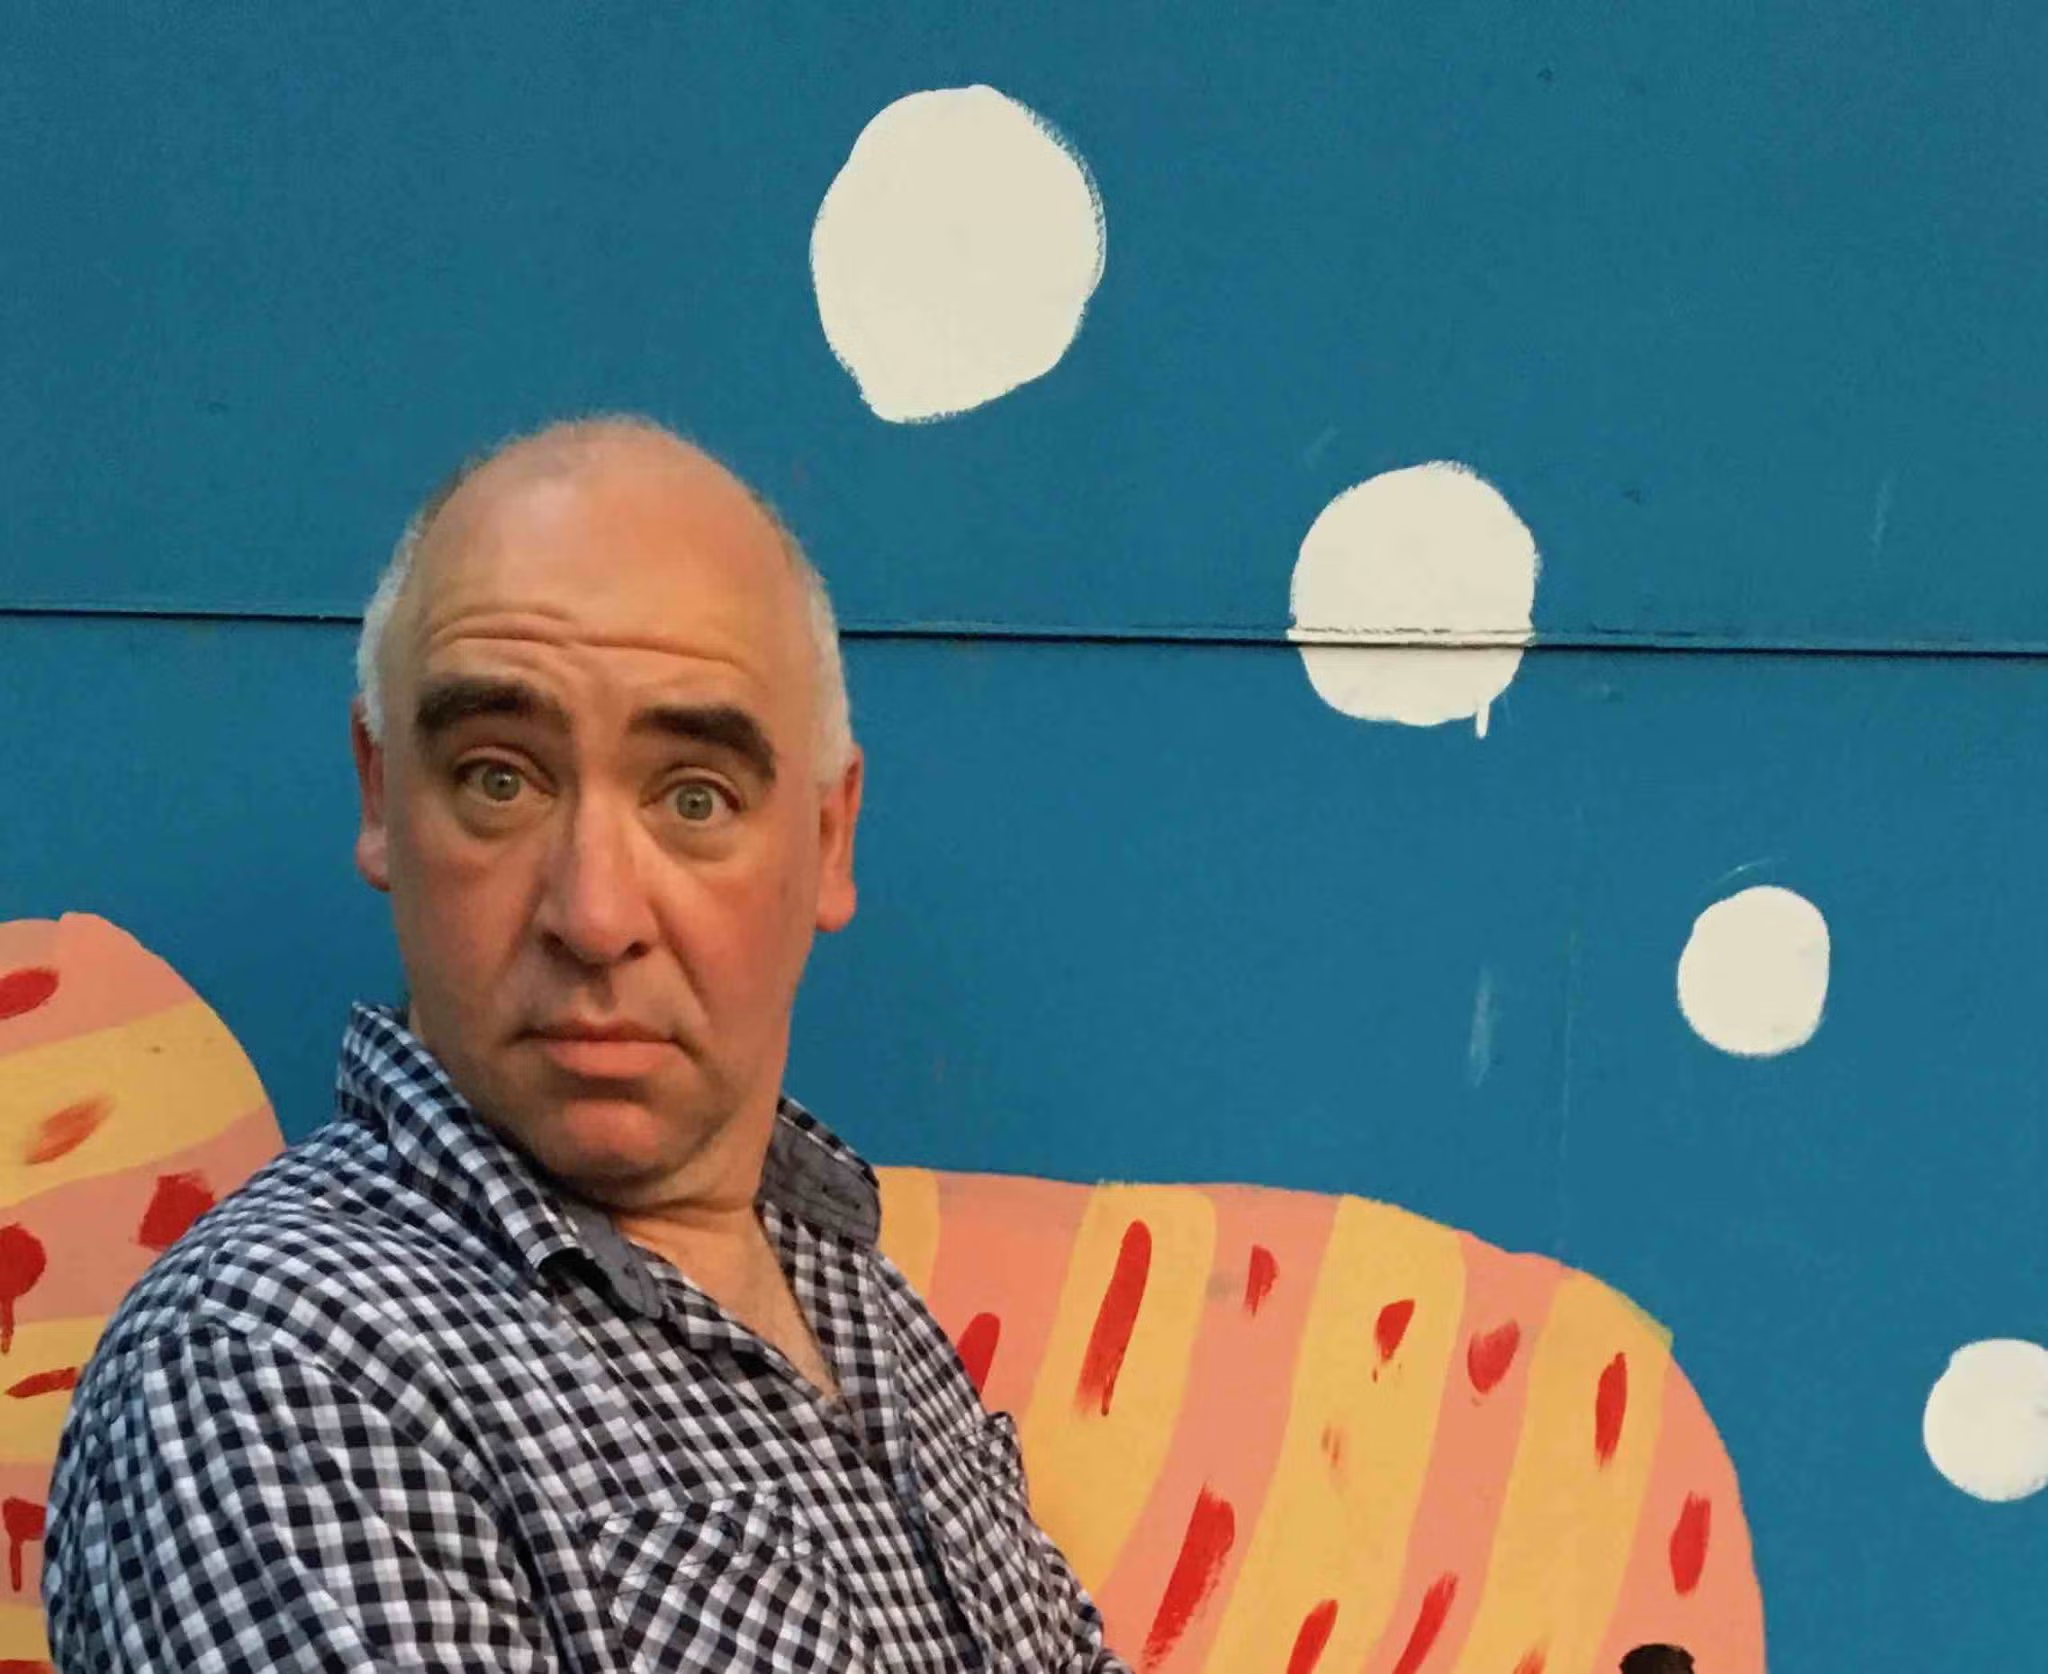
\includegraphics[width=0.5\linewidth]{image.png}
        \caption{Guess who?}
        \label{fig:placeholder}
    \end{figure}
        Benjamin : "Six feet tall and ruggedly handsome" - Prof. Doug Shaw, sometime in the 21st century. I probably don't require a reason for this. \color{djs}Early, early, 21st century\color{black}
        \color{blue}    RW: sometimes facts speak for themselves. \color{black}
        \newline Aadya: "RAWR" - Prof. Shaw...I look forward to witnessing this again one day \\
        \color{blue} RW: Aadya, please do not encourage this LOL. That was single-handedly the most weird thing I have ever seen this man do, and well I've known him for only several years, but I still think that speaks volumes after hearing the same 11 lectures five times! (Gah sorry about the run on sentence there!)
        \color{djs}I have no memory of what this refers to.\color{black}
        
         ANYWAYS! It was a real pleasure being your undergrad TA you all! I really think you guys put forth some \textbf {very} high quality work that I hope you are proud of. Whatever comes next for you all, please stay curious and I wish you the best! - Rachel \color{black}

         \color{djs} I really liked working with you all. I loved how you rolled with me whether I was doing hard math, easy math, or just rambling on. Thank you for teaching me to do things with Overleaf that I've never done. I hope you all have a great fall!\color{black}
        
    \end{solution}
\end{enumerate}
\end{document}